%& /home/emendoza/.config/emacs/.local/cache/org/persist/ee/420a54-8f37-40c0-b135-993ab30f9107-c4f7dccb7eaa21508c93c76d7c2f76f8
% Created 2025-10-21 Tue 12:56
% Intended LaTeX compiler: pdflatex
\documentclass[11pt]{article}
\usepackage[utf8]{inputenc}
\usepackage[T1]{fontenc}
\usepackage{amsmath}
\usepackage{amssymb}
\usepackage{capt-of}
\usepackage{hyperref}
\usepackage{em-mathtools}
\usepackage[a4paper,margin=2cm]{geometry}

%% ox-latex features:
%   !announce-start, !guess-pollyglossia, !guess-babel, !guess-inputenc, caption,
%   maths, image, !announce-end.

\usepackage{capt-of}

\usepackage{amsmath}
\usepackage{amssymb}

\usepackage{graphicx}

%% end ox-latex features


% end precompiled preamble
\ifcsname endofdump\endcsname\endofdump\fi

\author{Euan Mendoza}
\date{\today}
\title{LDE Quantum Algorithm Note}
\hypersetup{
 pdfauthor={Euan Mendoza},
 pdftitle={LDE Quantum Algorithm Note},
 pdfkeywords={},
 pdfsubject={},
 pdfcreator={},
 pdflang={English}}
\begin{document}

\maketitle
\tableofcontents

Let \(\F\) be a field (either \(\R\) or \(\C\)), and \(\F^{n}\) is a \(n\)-dimensional vector space over \(\F\).
\section{Summary and Key Ideas}
\label{sec:orge8227c5}
\begin{itemize}
\item Quantum computers can numerically solve LDE's in \(O(\log n)\) time where \(n\) is the dimension of a vector space, which takes \(O(n^{3})\) time classically.
\item This provides an exponential speed up which is due to quantum computers being able to efficiently solve systems of linear equations.
\item This speedup has some caveats, such as whether an exponential speedup for solving linear differential equations outweighs the costs of using quantum computers in the first place. Is it even that hard to solve LDE's classically or is the performance manageable (is waiting a couple hours for a computer to run ok).
\item How much time does it take to solve an LDE on a classical CAS like SageMath?
\item The cost of decomposing a non-unitary matrix as a product of unitaries. Computational cost of Gram-Schmidt?
\end{itemize}
\section{The Algorithm}
\label{sec:org9d4f238}
Our goal is to solve the Harmonic oscilator equation using a quantum algorithm,

\begin{equation}
\label{eqn:harmonic}
f''(x) + \omega^{2}f(x) = 0
\end{equation}
with initial conditions \(f(x) = 1, f''(x) = 1\). This can be rewritten as follows,

Let \(\alpha = f(x)\) and \(\beta = f'(x)\). By rewriting Equation \ref{eqn:harmonic} as \(f''(x) = \omega^{2}f(x)\) we obtain the following, \(\frac{d}{dx}\beta = f''(x) = -\omega f(x)\). For a vector \(v = \begin{bmatrix}\alpha \\ \beta \end{bmatrix}\), we obtain the following differential equation.

\begin{equation}
\frac{d}{dx} v = Av
\end{equation}

where

\begin{equation}
A = \begin{bmatrix}0 & 1\\ -\omega^{2} & 0\end{bmatrix}
\end{equation}

This equation can be solved symbolically to give us the following equation,

\begin{equation}
v(x) = e^{Ax}v(0)
\end{equation}
where \(v(0) = \begin{bmatrix}1 \\ 1\end{bmatrix}\) as per our initial equations.

Notice that when the Harmonic frequency \(\omega = 1\), our matrix \(A\) is unitary, in this case we denote the matrix \(A = U\).

We can numerically approximate \(v(x)\) to an approximation order \(k\) by truncating it's Taylor series as follows,

\begin{equation}
v(x) \approx \sum^{k}_{m=0} \frac{(Ut)^{m}}{m!}v(0)
\end{equation}
\subsection{The Quantum Circuit}
\label{sec:org56173b6}
\subsubsection{Goal}
\label{sec:org4a16c94}
Let \(A = \begin{bmatrix}0 & 1\\ -1 & 0\end{bmatrix}\), and \(u = f(0) = \begin{bmatrix}1\\ 1\end{bmatrix}\). Then we want to solve the equation,

\begin{equation}
f(t)\approx \sum^{k}_{m=0}\frac{(At)^{m}}{m!}f(0)
\end{equation}

This equation can be described by quantum states as follows. Let \(\ket{u}=\sum_{j\in \{0,1\}}\frac{u_{j}}{||u||}\ket{j}=\ket{+}\), and since \(A\) is unitary \(||A||=1\), which we can denote \(U=A\).

\begin{equation}
\ket{f(t)}\approx \sum^{k}_{m=0}\frac{||u||(Ut)^{m}}{m!}\ket{u}
\end{equation}

Then if we set a constant \(c_{m=||u||\frac{t^{m}}{m!}\), we can obtain the following equation which we claim can be simulated efficiently on a quantum computer.

\begin{equation}
\ket{f(t)}\approx \frac{1}{c^{4}}\sum^{k}_{m=0}c_{m}U^{m}\ket{u}
\end{equation}
where \(c = \sqrt{\sum c_{m}}\).
\subsubsection{{\bfseries\sffamily TODO} The Circuit}
\label{sec:orgcaffe30}
Let \(U_{u}\) be a unitary matrix that turns the state \(\ket{\varphi}\) into \(\ket{u}\) and \(V\) is the following \(k+1\times k+1\) matrix,

\begin{equation}
V = \frac{1}{c^{2}}\begin{bmatrix}
\sqrt{c_{0}} & Q & Q & Q & Q \\
\sqrt{c_{1}} & Q & Q & Q & Q \\
\sqrt{c_{2}} & Q & Q & Q & Q\\
\vdots       & Q & Q & Q & Q\\
\sqrt{c_{k}} & Q & Q & Q & Q
\end{bmatrix}
\end{equation}
where \(Q\) pads \(V\) to make it into a unitary.

\begin{figure}[htbp]
\centering
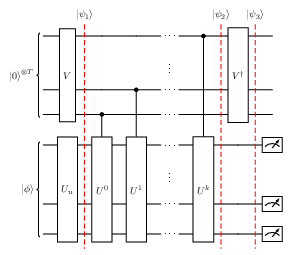
\includegraphics[width=7cm]{../figures/circuit.png}
\caption{\label{fig:circuit}The quantum circuit for solving the harmonic oscillator LDE}
\end{figure}
\begin{enumerate}
\item Encoding:
\label{sec:orga6b9273}
The circuit shown in Figure \ref{fig:circuit} has \(T=\log k\) ancilla qubits and a state \(\ket{\varphi}\), with state \(\ket{\psi_{in}}= \ket{0}^{\otimes T}\otimes \ket{\varphi}\). \(U_{u}\) turns \(\ket{\varphi}\) into \(\ket{u}\), and \(V\) leaves the system in the following state,

\begin{equation}
\ket{\psi_{1}} = \frac{1}{c^{2}}\sum^{k}_{m=0}\sqrt{c_{m}}\ket{m}\otimes\ket{u}
\end{equation}
\end{enumerate}
\section{Linear Differential Equations Background}
\label{sec:orgec2f689}

Recall that a differential equation that is written in terms of it's derivative. For example Schrodinger's equation is a differential equation,

\begin{align}
i\hbar \frac{\partial}{\partial t} \ket{\Psi(t)} = \hat{H}\ket{\Psi(t)}
\end{align}

A linear differential equation (LDE) is an equation where each derivative

\begin{align}
c_{0}f(x) + c_{1}\frac{df(x)}{dx} + c_{2}\frac{df^{2}(x)}{dx^{2}}\cdots c_{k-1}\frac{df^{k-1}(x)}{dx^{k-1}} + c_{k} = 0
\end{align}

Solving LDE's is incredibly important in material science, physics and economics.

Since solving differential equations plays such an important role in many fields of mathematics, science and economics, there are several tools that are classically well suited to solving differential equations.
\section{Differential Equations and Computation}
\label{sec:orge310529}

Differential equations form the backbone of many real world tasks in material science and quantitative finance. Therefore in computational algebra, there has been many different methods studied to efficiently solve differential equations. 

One of the first problems is understanding what it means to be \emph{efficient} in solving linear differential equations. There are many different approaches to solving LDE's where efficiency differs depending on the use case. They can be solved symbolically/algebraically or numerically for example.

There are several computer algebra systems that are quite good at solving differential equations, such as sagemaths, USyd Magma, Wolfram Mathematica and Matlab for example.
\subsection{Quantum Advantage}
\label{sec:orga09fadd}

\begin{itemize}
\item \href{https://www.wolfram.com/solutions/industry/materials-science/}{Mathematica use in material science}
\end{itemize}
\end{document}
